\documentclass[10pt]{article}
\usepackage{fixltx2e}
\usepackage[orthodox,l2tabu,abort]{nag}

% Page layout
\usepackage[landscape,margin=0.5in]{geometry}
\usepackage{multicol}
\usepackage{xcolor}

\usepackage{bbm}
\usepackage{amsmath}
\usepackage{amssymb}
\usepackage{graphicx}
\usepackage{amsfonts}
\usepackage{amsthm}


\usepackage{tikz}
\usetikzlibrary{calc}
\usetikzlibrary{arrows.meta}

% Title area
\usepackage{titling} % Allows for use of date, author, etc. after \maketitle
% Ref: http://tex.stackexchange.com/questions/3988/titlesec-versus-titling-mangling-thetitle
\let\oldtitle\title
\renewcommand{\title}[1]{\oldtitle{#1}\newcommand{\mythetitle}{#1}}
\renewcommand{\maketitle}{%
{\begin{center}\Large \mythetitle\end{center}}
}

% Document divisions
\usepackage{titlesec}
\setcounter{secnumdepth}{0}
\titlespacing{\section}{0pt}{0pt}{0pt}
\titlespacing{\subsection}{0pt}{0pt}{0pt}
\usepackage{nopageno} % To keep \section from resetting page style

\setlength{\parindent}{0pt} % disabling indentation by default

% Lists
\usepackage{enumitem} % for consistent formatting of lists
\newlist{ttdesc}{description}{1}
\setlist[ttdesc]{font=\ttfamily,noitemsep}
\usepackage{calc} % for \widthof

% Code
\usepackage{listings}
\lstset{language=[LaTeX]TeX,%
  basicstyle=\itshape,%
  keywordstyle=\normalfont\ttfamily,%
  morekeywords={part,chapter,subsection,subsubsection,paragraph,subparagraph}%
  }

\usepackage{lipsum}

\title{Complex Inner Product}
\author{Gabriele Carcassi}
\date{2015}

\begin{document}
\begin{multicols}{3}
\maketitle

\section{Inner product}

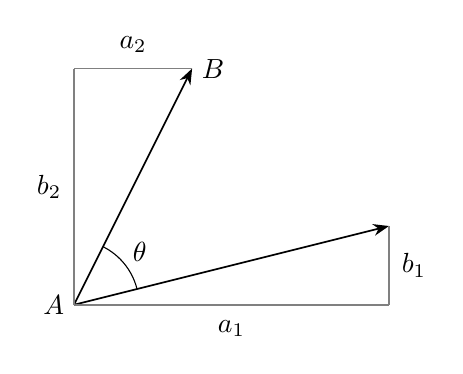
\begin{tikzpicture}[scale=1]
    
    
    \tikzstyle{help line}=[semithick,color=gray]
    \tikzstyle{vector}=[-Stealth,semithick,color=black]
    \tikzstyle{guideline}=[semithick,color=gray]
    \tikzstyle{guideline text down}=[black,below=2pt]
    \tikzstyle{guideline text right}=[black,right=1pt]
    \tikzstyle{guideline text up}=[black,above=2pt]
    \tikzstyle{guideline text left}=[black,left=1pt]
    %\draw[style=help line,step=2cm] (-2.5,-2.5) grid (2.5,2.5);
    % Draw a1 + b1 i
	\draw[style=vector] (0,0) -- (4,1);
	\draw[style=guideline] (0,0) -- node[style=guideline text down] {$a_1$} (4,0);
	\draw[style=guideline] (4,0) -- node[style=guideline text right] {$b_1$} (4,1);

    % Draw a2 + b2 i
	\draw[style=vector] (0,0) -- (1.5,3);
	\draw[style=guideline] (0,0) -- node[style=guideline text left] {$b_2$} (0,3);
	\draw[style=guideline] (0,3) -- node[style=guideline text up] {$a_2$} (1.5,3);

%    \draw (0,0) -- (1,0) arc(0:30:3mm);
%    \draw (15:2mm) node {$\alpha$};
\coordinate [label=left:$A$] (A) at (0,0);
\coordinate [label=right:$B$] (B) at (1.5,3);

%\draw[red,line width=1mm] let \p1 = ($(B)-(A)$) in (A) -- ++(45:({veclen(\x1,\y1)}););
%\draw (A) -- (B);
\draw let \p1 = (0,0),    % Center
          \p2 = (4,1),    % First vector
          \p3 = (1.5,3),  % Second vector
          \n1 = {0.2},    % Position of arc on first vector
          \p4 = ($(\p1)!\n1!(\p2)$),    % Point where the arc starts
          \n2 = {atan2(\y2,\x2)},       % First angle
          \n3 = {atan2(\y3,\x3)},       % Second angle
          \n4 = {veclen(\y4,\x4)},       % Arc radius
          \n5 = {\n2 + (\n3 - \n2) / 2},       % Mid angle
          \n6 = {\n4 + 7}       % Label radius
           in (\p4) -- ++(\p1) arc   (\n2:\n3:\n4) node at(\n5:\n6) {$\theta$} ;

\end{tikzpicture}

\begin{align*}
\overline{c_2} c_1 &= (a_2 - b_2 i) (a_1 + b_1 i) \\
&= a_1 a_2 + b_1 b_2 + \frac {a_1 b_2 - a_2 b_1}{i} \\
&= r_2 e^{-i\theta_2} r_1 e^{i\theta_1} \\
&= r_1 r_2 e^{-i\theta} \\
&= r_1 r_2 cos(\theta) + \frac {r_1 r_2 sin(\theta)}{i} \\
&= c_1 \cdot c_2 + \frac {c_1 \wedge c_2}{i} \\
\end{align*}

\section{Imaginary part}

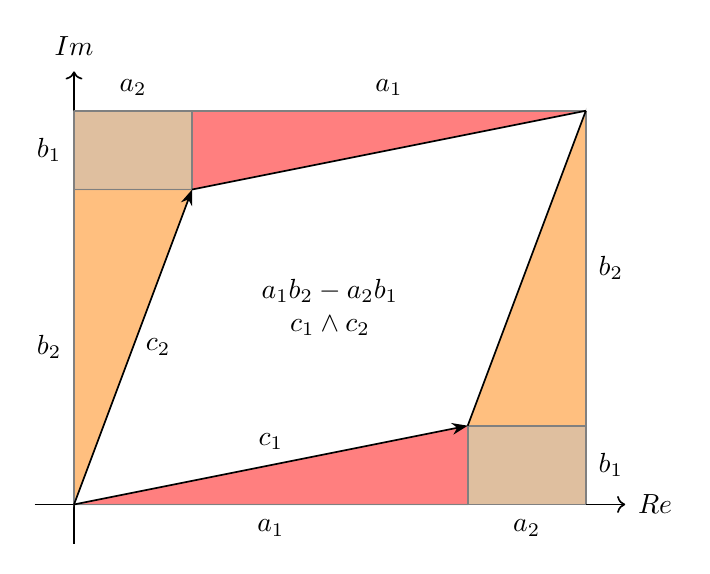
\begin{tikzpicture}[scale=1]
    \tikzstyle{axis}=[->,semithick,color=black]
    \tikzstyle{vector}=[-Stealth,semithick,color=black]
    \tikzstyle{parallel}=[semithick,color=black]
    \tikzstyle{guideline}=[semithick,color=gray]
    \tikzstyle{guideline text down}=[black,below=2pt]
    \tikzstyle{guideline text right}=[black,right=1pt]
    \tikzstyle{guideline text up}=[black,above=2pt]
    \tikzstyle{guideline text left}=[black,left=1pt]

	\coordinate (a_1) at (5,0);
	\coordinate (b_1) at (0,1);
	\coordinate (v_1) at ($(a_1)+(b_1)$);

	\coordinate (a_2) at (1.5,0);
	\coordinate (b_2) at (0,4);
	\coordinate (v_2) at ($(a_2)+(b_2)$);

    % Axis
	\draw[style=axis] (-0.5,0) -- ($(a_1)+(a_2)+(0.5,0)$) node[style=guideline text right] {$Re$};
	\draw[style=axis] (0,-0.5) -- ($(b_1)+(b_2)+(0,0.5)$) node[style=guideline text up] {$Im$};


    \filldraw[gray,fill=red,opacity=0.5](0,0)--(a_1)--(v_1)--cycle;
    \filldraw[gray,fill=red,opacity=0.5](v_2)--($(b_1)+(v_2)$)--($(v_1)+(v_2)$)--cycle;
    \filldraw[gray,fill=orange,opacity=0.5](0,0)--(b_2)--(v_2)--cycle;
    \filldraw[gray,fill=orange,opacity=0.5](v_1)--($(v_1)+(a_2)$)--($(v_1)+(v_2)$)--cycle;
    \filldraw[gray,fill=brown,opacity=0.5](b_2)--(v_2)--($(b_1)+(v_2)$)--($(b_1)+(b_2)$)--cycle;
    \filldraw[gray,fill=brown,opacity=0.5](a_1)--(v_1)--($(a_2)+(v_1)$)--($(a_1)+(a_2)$)--cycle;

    % Bottom
	\draw[style=guideline] (0,0) -- node[style=guideline text down] {$a_1$} (a_1);
	\draw[style=guideline] (a_1) -- node[style=guideline text down] {$a_2$} ($(a_1)+(a_2)$);
	\draw[style=guideline] (v_1) -- ($(v_1)+(a_2)$);

    % Left
	\draw[style=guideline] (0,0) -- node[style=guideline text left] {$b_2$} (b_2);
	\draw[style=guideline] (b_2) -- node[style=guideline text left] {$b_1$} ($(b_2)+(b_1)$);
	\draw[style=guideline] (v_2) -- ($(v_2)+(b_1)$);

    % Top
	\draw[style=guideline] ($(b_2)+(b_1)$) -- node[style=guideline text up] {$a_2$} ($(v_2)+(b_1)$);
	\draw[style=guideline] ($(v_2)+(b_1)$) -- node[style=guideline text up] {$a_1$} ($(v_1)+(v_2)$);
	\draw[style=guideline] (b_2) -- (v_2);

    % Right
	\draw[style=guideline] ($(a_1)+(a_2)$) -- node[style=guideline text right] {$b_1$} ($(v_1)+(a_2)$);
	\draw[style=guideline] ($(v_1)+(a_2)$) -- node[style=guideline text right] {$b_2$} ($(v_1)+(v_2)$);
	\draw[style=guideline] (a_1) -- (v_1);

    % Draw a1 + b1 i
	\draw[style=vector] (0,0) -- node[style=guideline text up] {$c_1$} (v_1);
	\draw[style=vector] (0,0) -- node[style=guideline text right] {$c_2$} (v_2);
	\draw[style=parallel] (v_1) -- ($(v_1)+(v_2)$);
	\draw[style=parallel] (v_2) -- ($(v_1)+(v_2)$);
	\draw[align=center] ($0.5*(v_1)+0.5*(v_2)$) node {$a_1 b_2 - a_2 b_1$ \\ $c_1 \wedge c_2$};


\end{tikzpicture}

\begin{align*}
Area&=(a_1+a_2)(b_1+b_2) - \textcolor{red}{a_1 b_1} - \textcolor{orange}{a_2 b_2}
- \textcolor{brown}{2 a_2 b_1}\\
&= a_1 b_2 - a_2 b_1 \\
\end{align*}

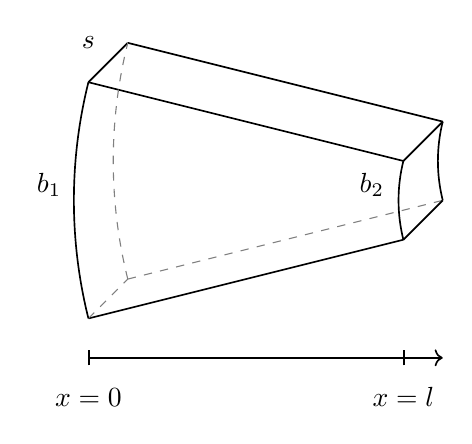
\begin{tikzpicture}
	% general shift to north east
	\coordinate (O) at (0.5,0.5);
	\draw[semithick] (0,0) -- (4,1);% bottom line in front
	\draw[dashed,color=gray] (O) -- ($(4,1)+(O)$);% bottom line in the back
	\draw[semithick] (0,3) -- (4,2);% top line in front
	\draw[semithick] ($(0,3)+(O)$) -- ($(4,2)+(O)$);% top line in the back
	\draw[semithick] (0,3) -- ($(0,3)+(O)$);% line to the back, top left
	\draw[semithick] (4,2) -- ($(4,2)+(O)$);% line to the back, top right
	\draw[semithick] (4,1) -- ($(4,1)+(O)$);% line to the back, bottom right
	\draw[dashed,color=gray] (0,0) -- (O);% line to the back, bottom left
	% the first angle is 180°+atan(0.25)
	% the second angle is 180°-atan(0.25)
	% the radius is sqrt(6^2+1.5^2)
	\draw[semithick] (0,0) arc (194.036:165.964:6.185);% left arc in front
	\draw[dashed,color=gray] (O) arc (194.036:165.964:6.185);% left arc in the back
	% the first angle is 180°+atan(0.25)
	% the second angle is 180°-atan(0.25)
	% the radius is 1/3*sqrt(6^2+1.5^2)
	\draw[semithick] (4,1) arc (194.036:165.964:2.062);% right arc in front
	\draw[semithick] ($(4,1)+(O)$) arc (194.036:165.964:2.062);% right arc in the back
	\draw (-0.5,1.7) node {$b_1$};
	\draw (3.6,1.7) node {$b_2$};
	\draw (0,3.5) node {$s$};
	\draw[|-,semithick] (0,-0.5) -- (4,-0.5);
	\draw[|->,semithick] (4,-0.5) -- (4.5,-0.5);
	\draw (0,-1) node {$x=0$};
	\draw (4,-1) node {$x=l$};
\end{tikzpicture}

\noindent Copyright \textcopyright{} \thedate{} \theauthor{}

\end{multicols}
\end{document}
